\documentclass{article}
\usepackage[brazilian]{babel}
\usepackage[utf8]{inputenc}
\usepackage{amsmath,amsfonts,amstext}


\usepackage{booktabs}
\usepackage{geometry}
\usepackage{graphicx}
\title{Implementação digital de um Minimoog}
\author{Bruno Figueira Lourenço \\ Jonathan Alis Salgado Lima}

\begin{document}
\maketitle

\section{Introdução}
O objetivo desse trabalho foi fazer uma implementação digital de um Minimoog em forma de \emph{plugin} VSTi.



\section{Arquitetura Geral do Sistema}
A implementação do Minimoog foi divida em duas partes, que correspondem às 
duas pastas na estrutura de diretórios do projeto:

\begin{itemize}
	\item \emph{src} - Contém as classes responsáveis por efetuar 
	a síntese de áudio propriamente dita. Foram implementadas diversas 
	unidades básicas. A classe \emph{Moog} conecta essas unidades básicas para 
	emular a estrutura do Minimoog. Esta pasta também contém um diretório 
	de testes (\emph{Tests}) para os blocos de síntese construídos.
	\item \emph{plugin} - Contém as classes responsáveis por fazer a 
	interface entre a síntese de áudio e a API VST.
\end{itemize}

\section{Síntese de Áudio}
Para implementar o Moog, optou-se por dividir em diversos blocos básicos, 
que representam cada um dos blocos que compõem o instrumento. Para isso, 
criou-se a classe \emph{BasicBlock} (\emph{basic\_blocks.h}) que representa 
uma unidade básica de síntese. A Figura \ref{fig:uml1} mostra o diagrama 
de classes correspondente.

\begin{figure}
\centering
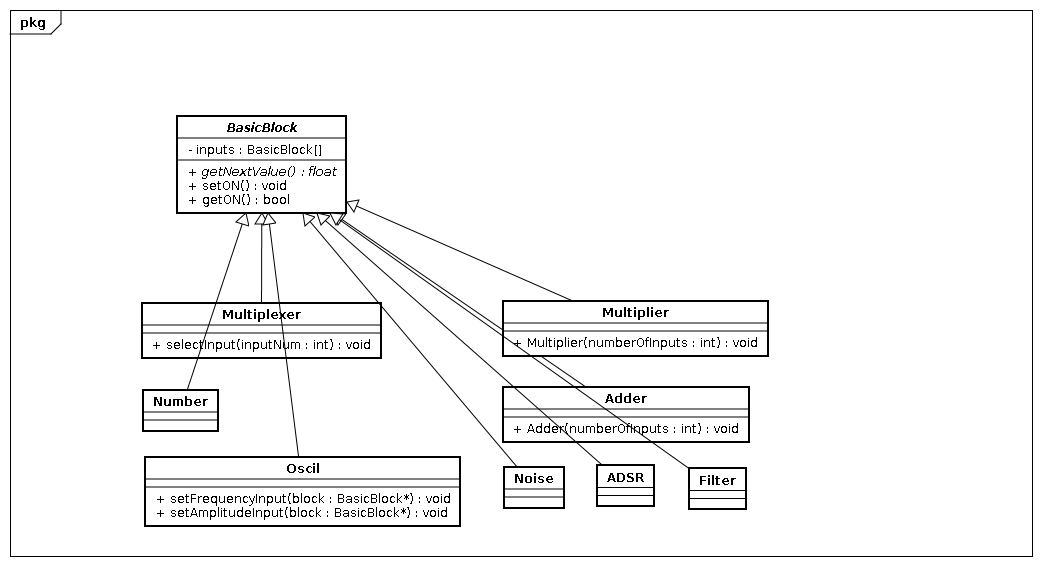
\includegraphics[scale=0.4]{Classes.png}\caption{Diagrama UML dos blocos básicos de síntese}\label{fig:uml1}
\end{figure}

Todos os blocos de síntese herdam da classe \emph{BasicBlock} e sobrescrevem 
o método \emph{getNextValue}, que é o responsável por obter a próxima 
amostra de áudio do bloco. A classe \emph{BasicBlock} também fornece métodos 
para ligar(\emph{getON} e \emph{setON}) e resetar (\emph{resetBlock}) a unidade.

Naturalmente, a semântica de ``ligar'' e ``resetar'' o bloco varia de unidade para unidade. 
Por exemplo, se desligarmos um \emph{Oscil} e chamarmos \emph{getNextValue}, a unidade 
retornará $0$. Já no caso da classe \emph{Filter}, desligar o filtro significa que não 
será feito processamento e o sinal será devolvido tal como recebido pelo filtro. 

Finalmente, através do método \emph{setInput} é possível usar um outro \emph{BasicBlock} 
como entrada para a unidade em questão. Por exemplo, a classe \emph{Oscil} recebe 
dois \emph{BasicBlock} como entrada, um representando a frequência e o outro 
a amplitude de oscilação.

Nas subseções seguintes descreveremos alguns aspectos das classes derivadas de \emph{BasicBlock}.

\subsection{\emph{Number}}
A classe numero(Number) serve para obtermos um número como sinal amostrado, usamos para obtermos um sinal de valor fixo. Ela não recebe nenhum outro bloco básico. Essa classe tem um atributo com o valor do número e a função que obtêm a próxima amostra simplesmente retorna esse número.
\subsection{\emph{Adder}}
Um somador(Adder) serve para podermos somar um número qualquer de sinais amostrados. Ao ser construída, deve-se passar o número de entradas, e ao usar deve indicar quais blocos básicos serão as entradas. Para obter a próxima amostra, são obtidas as próximas amostras de todos os blocos de entrada, somadas e esse valor é retornado.
\subsection{\emph{Multiplier}}
Um multiplicador(Multiplier) serve para podermos multiplicar um número qualquer de sinais amostrados. Funciona de forma análoga ao somador.
\subsection{\emph{Multiplexer}}
O multiplexador(Multiplexer) funciona como um seletor de uma das entradas. Ele também recebe um número arbitrário de blocos básicos ao ser construído, e também devem ser escolhidos quais são esses blocos. E tem uma função que escolhe qual bloco passará para a saída. A próxima amostra será a próxima amostra do bloco escolhido.
\subsection{\emph{Oscil}}
O oscilador(Oscilator) é um dos blocos mais importantes para esse sintetizador, ele que gera o sinal rico em harmônicos que será processado, manipulado e filtrado para obter o som sintetizado coom queremos.
Ele usa 2 blocos básicos que o controlam, a entrada de frequência e a entrada de amplitude, que são sinais que controlarão frequência e amplitude do oscilador. 
Há ainda uma função que controla qual tipo de onda que o oscilador usará. Esses tipos de onda estão estruturados em uma classe chamada Waveforms com os tipos de onda implementados, que são: triangular, dente de serra, quadrada, reta larga e reta estreita, que são colocados numa tabela usada pelo oscilador. Por fim o oscilador faz o table lookup dessa tabela  com interpolação linear.
A classe oscilador ainda faz sincronismos entre 2 osciladores. Se a opção pelo sincronismo estiver ativada um oscilador escravo é resetado no instante que o oscilador principal completa seu ciclo. Isso gera efeitos  bem interessantes que só sincronismo entre os osciladores proporcionam.

\subsection{Gerador de ruído}
O gerador de ruído (a classe Noise) não recebe nenhum bloco, ela gera 2 tipos de ruídos, o ruído branco e o ruído rosa.
o ruído branco é o ruído gerado por números aleatórios(nesse caso, as limitações da computação faz com que sejam números pseudo-aleatórios), que contém todas as bandas de frequência com a mesma intensidade.
o ruído rosa é o ruído que tem todas as bandas de frequência, mas com intensidades proporcionais ao inverso da frequência, ou seja, para maiores frequências menos vai ser a intensidade dela. A implementação usada foi a de [2].
\subsection{ADSR}
A classe ADSR é um controlador de envoltórias de amplitudo e frequência, essa sigla representa o atack, decay, sustain e release, que são respectivamente o tempo de ataque, decaimento, sustentação e relaxamento de uma envoltória....
\subsection{Filtro}

O filtro é uma implementacao digital dos filtros controlados por tensao(VCF)usados nos minimoogs, feito por Robert Moog. Esse filtro é uma construção em série de 4 filtros passa baixa implementados com circuitos RC, com resistencia variavel por tensao, podendo assim controlar a frequencia de corte,alem de uma realimentacao invertida multiplicada por um fator de qualidade (k) que varia de 0 a 4.
O comportamento dele é dependente do $k$, para $k=0$ ele atua como um passa baixa, com o crescimento de k, aparece uma elevacao 
cada vez mais acentuada na funcao de transferencia no valor da frequencia de corte, e quando k chega a 4 o filtro passa a oscilar.
Cada um dos 4 estagios do filtro pode ser representado pela funcao de transferencia

\begin{equation}\label{eq:(1)}
G(s) = \frac{\omega_c}{\omega_c+s}  
\end{equation}

Onde $\omega_c$ é a frequencia de corte em radianos, e $s$ é a variavel da Transformada de Laplace.
Ao serializar 4 esses filtros e introduzir uma realimentacao com o fator -k, a funcao de transferencia fica

\begin{equation}\label{eq:(2)}
 H(s) = \frac{G(s)^4}{1+k G(s)^4} 
\end{equation}


Para discretizar o filtro, usamos uma transformacao bilinear para obtermos uma G(z) a partir da G(s), 
com uma simples nova estimativa do valor $\omega_c$, chamaremos essa estimativa de $\omega_c$~.
substituindo s por $(\frac{2}{T})(\frac{z-1}{z+1})$ em (1), obtemos:

\begin{equation}\label{eq:(3)}
G(z) = b_0 \frac{1+z^{-1}}{1+a_1 z^{-1}}  
\end{equation}


Onde $b_0 = \frac{T \tilde{\omega_c}}{T \tilde{\omega_c}+2}$ e $a_1 = \frac{T \tilde{\omega_c} -2}{T\tilde{\omega_c} +2}$, onde $T$ é o período de amostragem.
Pela definicao de transformacao bilinear a pulsacao antitransformada $\tilde{\omega_c}$ do filtro digital é

\begin{equation}\label{eq:(4)}
\tilde{\omega_c} = b_0 \frac{2}{T} \tan({\frac{T \omega_c}{2}} ) 
\end{equation}

Bem com isso temos apenas a funcao de transaferencia de um estagio do filtro, mas precisamos da implementacao digital dele.
Fazendo $G(z) = \frac{Y(z)}{X(z)}$, e igualando a (3) e isolando Y(z), obtemos


\begin{equation}\label{eq:(5)}
Y(z) = b_0(X(z)+X(z)z^{-1})-a_1Y(z)z^{-1}
\end{equation}

Usando a transformada inversa $z$:

\begin{equation}\label{eq:(6)}
y(n)=b_0(x(n)+x(n-1))-a_1 y(n-1)  
\end{equation}


Esse é o nosso G(z), serializando 4 desses e acrescentando a realimentacao, o filtro fica implementado.

Em C++, foi feita a classe Filter, no arquivo Filter.cpp, que deriva da classe BasicBlock. Um objeto da classe Filter e criado com 3 BasicBlocks como entrada, sendo que o primeiro e o sinal que vai ser filtrado, a frequencia de corte do filtro e o fator de qualidade. Como o proximo valor da saida do filtro depende das entradas e saidas anteriores de cada um dos estagios, foi nescessario criar os atributos para guardar os valores anteriores e atualiza-los a cada solicitacao de novo valor para saida.

\section{A classe \emph{Moog}}

\section{VST}
O SDK para gerar plugins VST é distribuído pela Steinberg, e portanto, deve 
ser conseguido diretamente com a empresa. Nesta seção, temos como objetivo 
descrever como foi feito interfaceamento entre o arcabouço que foi montado 
para a síntese de áudio
\bibliographystyle{IEEEtran}
\bibliography{bibliografia}
\end{document}

